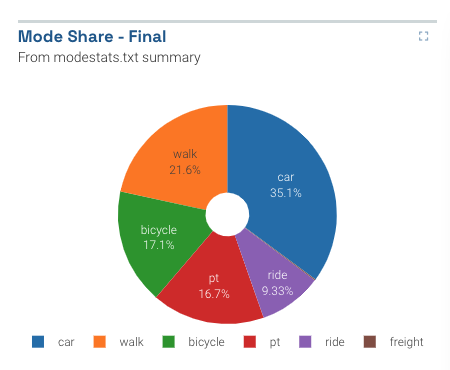
\includegraphics{assets/pie.png} \emph{It's a pie chart}

Sometimes a pie chart is all you need. Please remember to use them
sparingly; there are often better ways to depict aggregate data.

\hypertarget{usage}{%
\subsection{Usage}\label{usage}}

Pie charts can only be included as panels in \textbf{Dashboards}. See
Dashboard documentation for general tips on creating dashboard
configurations.

\begin{itemize}
\tightlist
\item
  Each pie chart panel is defined inside a \textbf{row} in a
  \texttt{dashboard-*.yaml} file.
\item
  Use panel \texttt{type:\ pie} in the dashboard configuration.
\item
  Standard title, description, and width fields define the frame.
\end{itemize}

\begin{center}\rule{0.5\linewidth}{0.5pt}\end{center}

\hypertarget{sample-dashboard.yaml-config-snippet}{%
\subsubsection{Sample dashboard.yaml config
snippet}\label{sample-dashboard.yaml-config-snippet}}

\begin{Shaded}
\begin{Highlighting}[]
\FunctionTok{layout}\KeywordTok{:}
\AttributeTok{  }\FunctionTok{row1}\KeywordTok{:}
\AttributeTok{    }\KeywordTok{{-}}\AttributeTok{ }\FunctionTok{type}\KeywordTok{:}\AttributeTok{ }\StringTok{\textquotesingle{}pie\textquotesingle{}}
\AttributeTok{      }\FunctionTok{title}\KeywordTok{:}\AttributeTok{ }\StringTok{\textquotesingle{}Mode Share\textquotesingle{}}
\AttributeTok{      }\FunctionTok{description}\KeywordTok{:}\AttributeTok{ }\StringTok{\textquotesingle{}From modestats.txt\textquotesingle{}}
\AttributeTok{      }\FunctionTok{width}\KeywordTok{:}\AttributeTok{ }\DecValTok{1}
\AttributeTok{      }\FunctionTok{dataset}\KeywordTok{:}\AttributeTok{ }\StringTok{\textquotesingle{}*modestats.txt\textquotesingle{}}
\AttributeTok{      }\FunctionTok{useLastRow}\KeywordTok{:}\AttributeTok{ }\CharTok{true}
\AttributeTok{      }\FunctionTok{ignoreColumns}\KeywordTok{:}\AttributeTok{ }\KeywordTok{[}\StringTok{\textquotesingle{}Iteration\textquotesingle{}}\KeywordTok{]}
\end{Highlighting}
\end{Shaded}

\begin{center}\rule{0.5\linewidth}{0.5pt}\end{center}

\hypertarget{pie-chart-properties}{%
\subsubsection{Pie chart properties}\label{pie-chart-properties}}

Pie chart properties:

\textbf{dataset:} String. The filepath containing the data. May include
wildcards * and ?.

\textbf{useLastRow:} true/false. If set to true, only the last row of
the datafile will be used to build the pie chart. For example, this is
useful for MATSim outputs which list every iteration's output, if you
are only in the final iteration.

\textbf{ignoreColumns:} Array of strings. List the column names of any
columns that should be left out of the pie chart (e.g.~Iteration).
Example: \texttt{{[}\textquotesingle{}Iteration\textquotesingle{}{]}}
